\chapter{Chromosome Nomenclature}
\label{ap:appendNom}

\begin{fquote}[Ludwig Wittgenstein]If people never did silly things, nothing intelligent would ever get done. \fqsource{{Austrian philosopher (1889 - 1951)}} \end{fquote} 

There is a standardized naming scheme or nomenclature to address the different areas in the genome defined by the International System for Human Cytogenetic Nomenclature (ISCN) \cite{iscn}. This naming scheme is used by the domain experts and found in the literature when addressing the parts of the genome. The history of chromosome nomenclature dates back to 1971 when a meeting in Paris decided the basic nomenclature for the bands in the chromosome. Hence, the nomenclature is often referred to as Paris nomenclature and some names have been adopted from French.

A chromosome is divided into two arms by the centromere: the p arm which stands for petit (meaning small in French)  is the longer arm and the arm q which stands for queue. The regions are named q1, q2, q3 or p1, p2, p3 starting from the centromere and moving towards the edges. Regions are often separated by specific and consistent landmarks which possess distinct morphological characters such as the ends of the chromosome arms, the centromere and certain bands. The regions are further divided into bands such as q11 (pronounced as ‘q-one-one’ not ‘q-eleven’). The bands are further divided into sub-bands such as q11.1 or even sub-sub bands such as q11.11. This naming scheme is hierarchical and irregular.

\begin{figure}[h!]
\centering
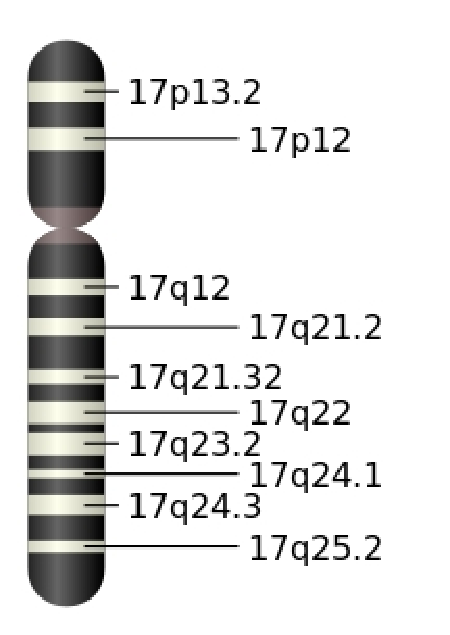
\includegraphics[width=0.4\textwidth]{figures/chromonomen}
\caption[Regions in chromosome 17 and resolution 400]{Nomenclature of Chromosome bands of Chromosome 17 in resolution 400.} \label{Fig:chromonomen}
\end{figure}

An example of chromosome nomenclature is shown in Figure \ref{Fig:chromonomen} which is an example case in chromosome 17. For example, area 17q21.32 means chromosome 17, arm ‘Q', region 21, band 3 and sub-band 2. It is important to note that length of each region, band and sub-band varies.

ISCN has also defined Ideograms for G-banding patterns for normal human chromosomes at five different resolutions \cite{iscn}. Five different resolutions of chromosomes mean that a chromosome is divided into different parts in different resolutions. In resolution 400, for example, the chromosome is divided into 393 different parts and in resolution 850, chromosome is divided in 862 different parts. With respect to the chromosome bands region q21 in resolution 400, for example, is divided into q21.1, q21.2, q21.31, q21.32 and q21.33 in resolution 850. However, region q22 in resolution 400 remains undivided in resolution 850 as well. The division of the chromosome bands is determined by the resolution of naming scheme which depends on the properties of the genome.